\chapter{Introduction a EMMA}
\label{ch:introduction}
% (cf loi de \cite{moore1965cramming}). 
%\cite{THOMPSON200620}

%Les échelles de temps sont radicalement opposées entre la cosmologie qui considère les temps les plus long de l'univers et les progrès informatiques qui vont à une vitesse exponentielle.
%Du fait de l'avancée rapide des moyens de calculs, les simulations numérique sont des produits possédant une valeur se dépréciant rapidement et doivent être considérées comme éphémère.

Nous avons vu dans la partie précédente qu'elles étaient les principales physiques à l’œuvre durant l'époque de réionisation.
L'objectif de cette partie est d'expliquer comment ces physiques sont modélisées et quelles sont les contraintes sur leurs implémentations.
On se concentrera particulièrement sur le cas du code de simulations numériques EMMA.

EMMA est un code à grille adaptative ou \ac{AMR} capable de simuler l'évolution de la matière noire, du gaz et de la radiation de manière auto-cohérente et dans un contexte cosmologique.
Son principal objectif est de simuler l'\ac{EoR} et sa description complète pourra être trouvée dans \cite{aubert_emma:_2015} en annexe \ref{pap:EMMA}.
J'ai été amené à interagir avec toutes les parties d'EMMA, et à en modifier quelques unes.
%Une de mes premières tâches à été l'introduction d'un modèle de formation et d'évolution stellaire (cf section \ref{sec:etoiles}).
%Ce modèle de formation stellaire se trouve au carrefour entre toute les physiques gérées par EMMA.
La première partie de ce chapitre sera consacrée à une rapide présentation générale du contexte dans lequel le développement d'EMMA est réalisé, puis à la présentation de la grille adaptative, qui va contraindre un certain nombre de choix par la suite.
L'objectif de la seconde partie est de fournir un aperçu des différentes techniques et moteurs physiques utilisés pour mieux appréhender les résultats obtenus à l'aide de ce code.
Dans la troisième partie je présenterai quelques contraintes matérielles dans l'exécution d'EMMA et également quelques développements que j'ai réalisé, entre autre une amélioration de la gestion des entrées/sorties.


%Comment modéliser la reionization?

\section{Aperçu des différents modèles numériques}
\label{sec:gridpart}
Un code de simulation cosmologique a pour vocation principale de suivre l'évolution de différents "fluides", comme la matière noire, la gaz, les étoiles et la radiation ou encore le champs magnétique.
Ces fluides sont de natures différentes et il n'y a pas de méthode unique permettant de suivre de manière optimale ces différentes physiques.
%On distinguera principalement deux catégories de fluides: les collisionnels et les non-collisionnels.
%La physique non-collisionnelle concerne les phénomènes qui n'interagissent pas par collision comme la matière noire, les étoiles ou la radiation. 
%La physique collisionnelle concerne qant à elle principalement l'hydrodynamique du gaz.
Il existe conceptuellement deux principales façons de suivre un fluide dans l'espace.
%Ces deux approches sont dites \emph{Eulérienne} ou \emph{Lagrangienne}.
%En lien direct avec ces deux familles de représentations physique, il existe deux principales familles de codes cosmologique% : les codes \ac{SPH} et les codes \ac{AMR}.

\paragraph{La représentation Lagrangienne} consiste à se placer au point de vue du fluide.
On considère une série d'éléments de fluide de masse fixe pouvant se déplacer et/ou se dilater dans l'espace.
Les codes utilisant ce type de représentation seront généralement associés avec une gestion de la physique sous forme de \emph{particules}.
Les codes dit \ac{SPH}, \ac{PIC} ou tree-code sont des représentants de cette catégorie.

%\paragraph{\ac{SPH} : } représente le gaz sous forme de particule de masse constante mais de taille variable.
%Notion d'arbre -> KDtree

\paragraph{La représentation Eulérienne} consiste à se placer au point de vue de l'espace.
On considère un élément d'espace et le bilan de matière entrant et sortant de chacune de ses interfaces.
On associera généralement les codes utilisant ce type de représentation avec une gestion de la physique sous forme de \emph{grille}.
Si la grille a une résolution dynamiquement variable, on parlera de grille \ac{AMR}.

%\paragraph{Code sur grille} : représente l'espace sous forme de cellules organisées sur une grille. 
%Notion d'arbre -> arbre AMR
%La représentation Lagrangienne la plus populaire (dans le domaine des simulations cosmologiques) est sans doute le \emph{Smouth Particle Hydrodynamics (SPH) }
%Les volumes cosmologiques étant généralement cubique, les éléments de grille le sont généralement aussi.
%historique
%avantage inconvénient AMR vs SPH
%introduction de la grille et de la méthode AMR

\paragraph{}
Un même code peut utiliser conjointement plusieurs de ces représentations.
Dans le cas présent, EMMA utilise une représentation Lagrangienne pour simuler la physique de la matière noire et des étoiles, et une représentation Eulérienne pour simuler le gaz et le rayonnement.

\subsection{Quelques codes de simulations cosmologiques}

EMMA s'inscrit dans une certaine variété de codes de simulations cosmologiques existants, en voici un bref aperçu.
Ces codes sont classés en fonction de leur façon de gérer l'hydrodynamique du gaz et on distinguera principalement les codes \ac{SPH} et les codes \ac{AMR}.

Parmi les représentants des codes \ac{SPH} on citera entre autre:
\begin{itemize}
\item GADGET \citep{springel_cosmological_2005}
\item GASOLINE2 \citep{2017arXiv170703824W}
\item PHANTOM \citep{2017arXiv170203930P}
\end{itemize}

Parmi les représentants des codes \ac{AMR} on citera entre autre:
\begin{itemize}
\item ART \citep{1997ApJS..111...73K}
\item FLASH \citep{0067-0049-131-1-273}
\item RAMSES \citep{teyssier_cosmological_2002}
\item ENZO \citep{bryan_enzo:_2014}
\item EMMA \citep{aubert_emma:_2015}
\end{itemize}

Il existe un troisième type de code hybride utilisant une maille mobile et adaptative, un représentant majeur de cette technique est le code AREPO \citep{2010MNRAS.401..791S}.

Il existe évidemment d'autre codes, et la majorité d'entre eux disposent de plusieurs déclinaisons en fonction de ce pour quoi ils sont utilisé.

Des projets comme le projet Santa Barbara \citep{1999ApJ...525..554F} ou le projet nIFTy \citep{sembolini_nifty_2015} visent à comparer les codes entre eux.
Certain projets \citep{2007MNRAS.380..963A, oshea_comparing_2005} se focalisent sur la comparaison des méthodes.
% les codes \ac{SPH} auront une meilleur conservation de la masse,
D'une manière générale, il en ressort qu'un code \ac{AMR} offre une meilleur conservation de l’énergie et est plus apte à gérer les chocs et les instabilités mais pourra souffrir de problèmes de diffusion numérique.
Les codes \ac{SPH} auront plus de facilités à représenter de larges contrastes de densité, la où l'\ac{AMR} nécessitera un nombre important de niveaux, mais souffrira de bruit dans les régions sous-dense.

EMMA utilise des concepts déjà existant, entre autre une gestion de la grille adaptative similaire à ART ou RAMSES (voir section \ref{sec_gestion_grille}).
Les moteurs physiques (vois section \ref{sec:solvers}) ont également fait leurs preuves, par exemple la gravitation est gérée de manière comparable à ART, le moteur hydrodynamique est similaire à celui de RAMSES et le moteur radiatif est une réécriture de ATON \citep{aubert_radiative_2008}.
EMMA a été développé dans l'idée d'utiliser les processeurs graphiques ou \ac{GPU} pour en utiliser au maximum leurs capacités de calculs.
L'avantage par rapport aux codes plus anciens, est que cet objectif a été définis dès le départ, alors que les autres codes se sont adapté à cette évolution de matériel.
Il en résulte l'utilisation de certaines techniques menant à une implémentation différente (voir section \ref{sec:gpu}).


%EMMA est largement inspiré de RAMSES \citep{teyssier_cosmological_2002}.
%Ce dernier est une référence reconnue dans le domaine  des simulations cosmologiques et utilise des principes éprouvés, et EMMA en utilise un bon nombre.
%Entre autre, la gestion de la grille le moteur hydrodynamique et le moteur radiatif sont similaires.
%Le développement d'EMMA vise à obtenir une expertise complète sur le fonctionnement de ce type de code.
%
%EMMA a cependant quelques différences fondamentale avec RAMSES.
%Il n'utilise pas le même langage: RAMSES est écrit en Fortran, EMMA en c.
%Le développement de RAMSES a débuté avant l'apparition des \ac{GPU} et a ensuite été adapté pour en utiliser les capacités de calcul.
%EMMA est développé avec cette idée dès le départ, ce qui permet l'utilisation de certaines techniques menant à une implémentation différente.

\section{Gestion de la grille}
\label{sec_gestion_grille}
%(nécessaire d'être positionné ici car la structure en arbre conditionne plusieur choix par la suite)

Un des concepts central de EMMA est sa grille adaptative.
Tout les moteurs physiques sont basés dessus et sa structure conditionne un certain nombre de choix par la suite.
C'est pourquoi nous allons la développer ici, avant de rentrer plus en détails dans l'implémentation des différents moteurs physiques.

\subsection{Grille régulière et AMR}
Avant d'aborder le concept de grille adaptative faisons un léger détour par l'exemple d'une grille fixe et régulière.
Dans le cas des simulations sur grille fixe, les données sont réparties en mémoire de façon ordonnée.
L'organisation en mémoire et la recherche de voisins sont relativement simple à gérer.
Les vecteurs sont alloués de manière statique et la recherche de voisins est basée sur un jeu d'indice assez simple.
Dans un espace en 3D, on accédera à une cellule contenant le point de coordonnées normées $(x,y,z)$ sur une grille de $N_x*N_y*N_z$ cellules, à l'aide de son identifiant Id dans le tableau en mémoire.

\begin{equation}
Id = i + j*N_x + k * N_x*N_y
\end{equation}
avec :
\begin{equation}
\begin{cases}
i=\lfloor x \rfloor \cdot N_x \\
j=\lfloor y \rfloor \cdot N_y \\
k=\lfloor z \rfloor \cdot N_z \\
\end{cases}
\end{equation}
ou $\lfloor a \rfloor$ représente la partie entière de $a$.

Les choses sont plus complexes dans le cas d'une grille adaptative.
La grille étant amenée à évoluer, il faut introduire des mécanismes permettant de construire ou détruire certaines de ses parties de façons dynamique.
Ces mécanismes vont totalement changer l'organisation de la grille.

Un exemple de grille \ac{AMR} générée par EMMA est présenté sur la figure \ref{fig:AMR}).
Un fonction de critères prédéfinis par l'utilisateur comme par exemple un seuil de densité la résolution de la grille peut être arbitrairement augmentée localement.
L'avantage de ce type de grille est d'économiser des ressources de calcul par rapport au cas d'une grille fixe, ou il faudrait beaucoup plus de cellules pour obtenir une résolution équivalente.

\begin{figure}
        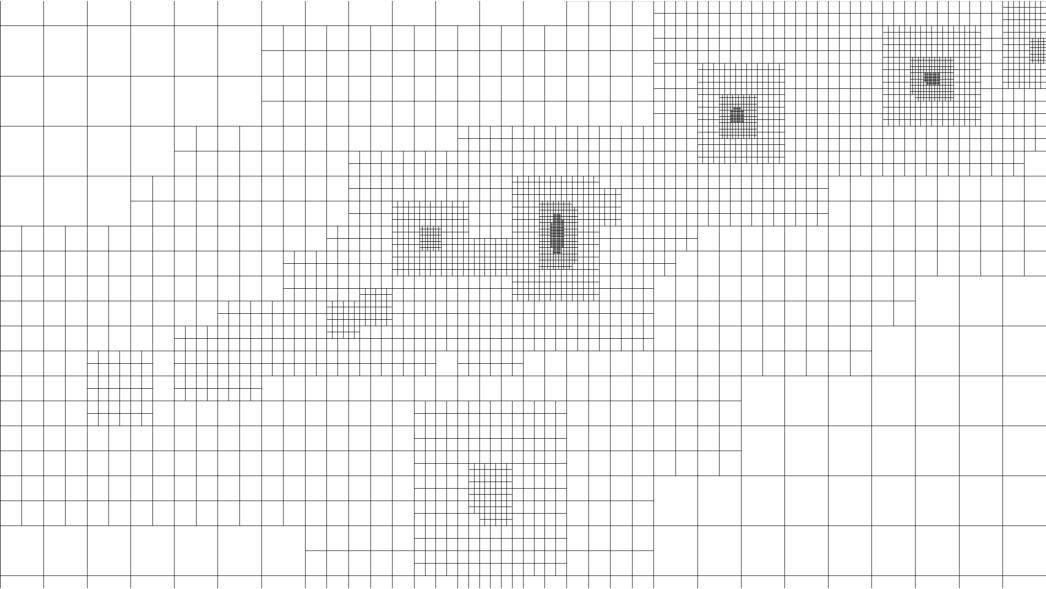
\includegraphics[width=.95\linewidth]{img/02/AMR.pdf} 
        \caption[Grille générée par EMMA]{Exemple de grille \ac{AMR} générée par EMMA. 
        La  résolution de la grille est augmentée arbitrairement dans les régions d'intérêts.
 		\label{fig:AMR}}
\end{figure}

\subsection{Maille adaptative}

Il existe deux grands groupes de mailles adaptatives.
Le premier groupe utilise une séries de grilles fixes imbriquées dites à "patch" (eg ENZO \cite{bryan_enzo:_2014}).
Chaque région raffinée sera représenté par une grille fixe spatialement liée à la grille de niveau supérieur.
Il est possible d'ajouter récursivement autant de niveaux que voulu et chacune de ces nouvelles grilles aura une résolution doublée par rapport à la précédente.

EMMA utilise un second groupe d'\ac{AMR} à base d'arbre de cellules. % fully threated tree description .
La base de cette représentation est de considérer que chaque cellule est associée à une grille fixe de taille $2 \times 2 \times 2$ que l'on nommera un oct, car décomposé en 8 cellules \citep{khokhlov_fully_1998-1}.
%sous parties qui sont elles même des cellules.
Et récursivement, chacune de ces cellules pourra à son tour être divisée et associée à un oct.
Il en résultera un arbre nommé octree, représenté sur la figure \ref{fig:octree}.

\begin{figure}
        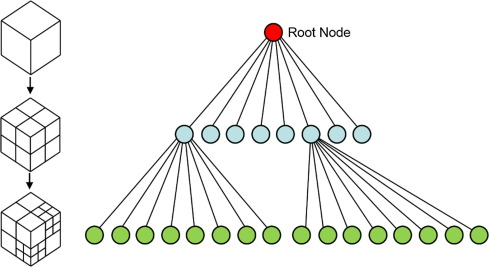
\includegraphics[width=.95\linewidth]{img/02/octree.jpg} 
        \caption[Grille AMR et son octree]{Représentation d'une grille AMR à gauche, et de son octree associé à droite. 
        Image extraite de \cite{SU201659}
     	\label{fig:octree}
}
\end{figure}

Pour créer la grille de base, il faudra d'abord créer une première cellule, et la forcer à raffiner.
Chacune de ces nouvelles cellules vont à leurs tours être raffinée.
Cette opération est répétée de manière récursive pour toutes les nouvelles cellules jusqu'à obtention d'une grille régulière de la taille désirée.
À chaque nouveau raffinement le nombre de cellule est multiplié par 8, le nombre de cellules d'un niveau entièrement raffiné est donc de:
\begin{equation}
N_{cells} = 2^{3L}
\end{equation}
où $L$ est le niveau de raffinement.

Il en résultera une grille régulière qui ne pourra pas être dé-raffinée par la suite.
Le niveau de cette grille sera appelé niveau de base.

\subsubsection{Les listes chaînées}
\label{sec:listechainee}
%il n'existe plus de lien direct entre la représentation de la grille en mémoire et la représentation de l'espace physique.
Comme la grille est amenée à évoluer, il n'existe plus de lien direct entre une position dans l'espace et une position en mémoire.
De plus le nombre d'éléments peut changer au cours du temps.
%Il faut donc conserver à la fois l'information de la position dans l'espace physique et dans l'espace mémoire.
En principe, on allouera une certaine quantité d'éléments en mémoire au début de la simulation, ce qui constituera une réserve, puis on viendra piocher dans cette réserve pour ajouter des éléments à la grille au fur et à mesure.
Comme un élément peut être ajouté n'importe où dans la grille, chaque élément devra conserver l'information de sa position en mémoire.
Ceci sera réalisé en les organisant sous forme de liste, et en stockant pour chaque élément, la position de l'élément précédent et celle de l'élément suivant dans cette liste.
En connaissant la position du premier élément de la liste, il est possible d'avoir accès à toutes la grille.
On appelle ce type de liste, des liste doublement chaînée.

L'octree est séparé en deux types de structures, les OCTs contenant l'information l'arbre à proprement parler, et les CELLs contenant l'information physique.
Le lien entre ces deux structures est schématisé sur la figure \ref{fig:octcell}.
On remarquera que les CELLs ne se voient pas entre elles et qu'il est nécessaire d'utiliser les OCTs pour déterminer leur voisinages.

\begin{figure}
        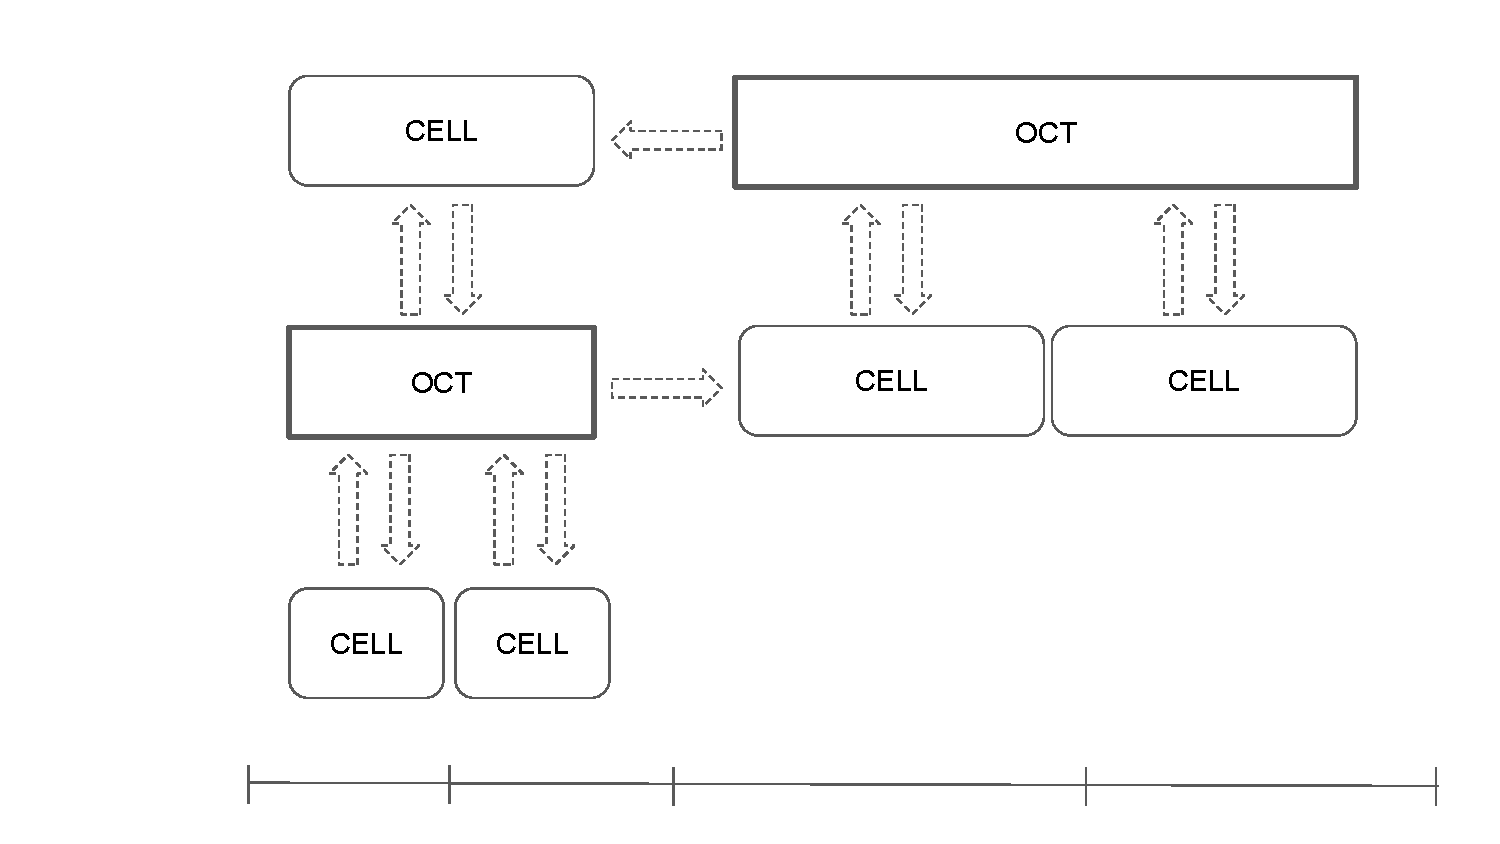
\includegraphics[width=.95\linewidth]{img/02/octcell.pdf} 
        \caption[OCT et CELL]{Représentation des lien entre OCT et CELL à 1 dimension.
        Les flèches représentent les pointeurs entre les structures.
        Le domaine 1D équivalent à cet arbre est représenté au bas de la figure.
     	\label{fig:octcell}
}
\end{figure}


\subsubsection{La structure CELL}
\label{sec:CELL}
Les cellules contiennent l'information physique de la grille (densité, pression, température, etc...).
Chaque cellule peut, sous certaines conditions, être associée un OCT pour augmenter la résolution localement.
La CELL qui n'a pas d'OCT père est appelée cellule racine, en pratique il n'y en a qu'une seule, contenant l'ensemble de l'espace de la grille..
Une CELL qui n'a pas d'OCT enfant est dite cellule feuille.
L'information de la position de la cellule dans l'OCT parent est contenue dans son identifiant (allant de 0 à 7).
Les CELLs contiennent également la liste chaînée de particules.
La structure minimale d'une CELL de EMMA est présenté sur le listing \ref{lst:cell}.

\begin{lstlisting}[float=bth,language=C,frame=tb,caption={La structure CELL de EMMA},label=lst:cell]
struct CELL{
  int id;            // permet de determiner la position de la cellule dans l'oct
  struct OCT *parent // l'oct pere de la cellule
  struct OCT *child; // si child est different de NULL alors la cellule est raffinee et child point vers l'oct enfant
  struct PHYSIC *data; // pointeur vers la partie physique
  struct PARTICLE *part; // pointeur vers la chaine de particules.
};
\end{lstlisting}


\subsubsection{La structure OCT}
%Pour créer un lien entre elle, il est nécessaire de stocker l'information de voisinage.
Les OCTs contiennent l'information relatives à la structure de la grille et permettent son raffinement.
Un OCT se trouve toujours entre sa mère et ses filles : il contient nécessairement un pointeur vers sa CELL mère ainsi qu'un tableau de huit CELLs filles.
Les OCTs contiennent également l'information sur le voisinage et chacun d'eux dispose de six pointeurs vers les CELLs voisines.
La génération de conditions périodiques (généralement utilisées en cosmologie) se fait de manière naturelle en faisant pointer tous les voisins de l'OCT de la CELL racine vers lui même.
La structure minimale d'un OCT de EMMA est présentée sur le listing \ref{lst:oct}.
%L'information spatiale est aussi contenue dans les OCT, 
\begin{lstlisting}[float=bth,language=C,frame=tb,caption={La structure OCT de EMMA},label=lst:oct]
struct OCT{
  struct CELL cell[8]; // les 8 cellules de l'oct
  struct CELL *nei[6]; // pointeurs sur les cellule voisines
  struct CELL *mother; // cellule mere
  struct OCT *next;    // oct suivant dans la liste chainee
  struct OCT *prev;    // oct precedent dans la liste chainee
  int level;           // niveau de l'oct
};
\end{lstlisting}


\subsubsection{La structure PARTICULE}
\label{sec:PART}

Nous verrons dans la section \ref{sec:solverDM} qu'une partie de la physique est résolue sous forme de particule.
Il est donc nécessaire d'ajouter un champs de particule à la grille \ac{AMR}.
Comme les OCT, les particules utilisent une représentation sous forme de liste chaînée, et chaque cellule dispose de sa propre liste chaînée de particules.
Lors de raffinement cette liste devra être découpée et distribuée entre les nouvelles cellules crées.
Une particule est essentiellement caractérisée par sa position, sa masse et sa vitesse.
On ajoutera à ceci son statut, qui sera utilisé pour différentier les particules de matière noire des particules stellaires. 
Le listing \ref{lst:part} présente la structure minimale d'une particule dans EMMA.


\begin{lstlisting}[float=bth,language=C,frame=tb,caption={La structure PARTICULE de EMMA},label=lst:part]
struct PART{
  REAL3 x;  // vecteur position
  REAL3 v;  // vecteur vitesse
  struct PARTICULE *next;  // particule suivante
  struct PARTICULE *prev;  // particule precedente
  int idx;  // identifiant unique
  int  isStar;  // matiere noire ou etat de l'etoile
  REAL t;       // instant de creation
  REAL mass;    // masse
};
\end{lstlisting}



\subsection{Gestion du raffinement}
\label{sec:raffinement}
%différentes condition de raffinement.\\
%sur la matière noire\\
%semi Lagrangienne\\
%sur le gradient d'ionization\\
%sur le gradient de densité (shock)\\

\subsubsection{En pratique}
Le raffinement se fera en trois temps:

\begin{itemize}
\item Dans un premier temps le code va passer en revue toutes les cellules d'un niveau, et les marquer comme "à raffiner" si une première condition physique est respectée (cf section \ref{sec:condraf}.

\item Une fois tout le niveau passé en revue, le code va ensuite faire une série de $N_{buffer}$ passages sur tout le niveau en marquant à chaque fois toutes les cellules voisines des cellules précédemment marquées.
Cette zone de $N_{buffer}$ cellules autour des zones soumises à la condition physique de raffinement sera appelée le "buffer de raffinement".
Ce tampon a pour but d’élargir la zone de raffinement et ainsi permettre une transition douce entre les niveaux.
De plus il ne sera autorisé à n'avoir qu'un seul niveau de décalage au maximum lors des transitions.

\item Une fois les cellules respectant ces deux conditions marquées, le raffinement est effectué.
\end{itemize}

%En pratique le raffinement d'une cellule se fera en lui associant un OCT.
%*child pointera alors vers le dernier OCT libre de la liste chaînée.

\subsubsection{Condition de raffinement}
\label{sec:condraf}

Il est possible de définir arbitrairement une condition de raffinement en fonction de la physique que l'on cherche à étudier.
Par exemple, dans des tests unitaires de type sphère de Stömgren (cf \ref{sec:stromgren}) ou explosion de Sedov (cf \ref{sec:sedov}), on marquera les cellules qui sont soumises à un gradient d'ionisation ou de densité supérieur à un certain seuil pour suivre l'évolution du front.
Dans le cas de simulations cosmologique, on utilisera généralement une condition en densité dite semi-Lagrangienne.
C'est a dire qu'une cellule sera marquée comme "à raffiner" si la masse de matière noire (ou de gaz) qu'elle contient est supérieur à huit fois la masse de matière noire (ou de gaz) moyenne d'une cellule de ce niveau.
%le deraffinement
On remarquera que la condition de raffinement ne prends pas en compte le fait qu'une cellule soit déjà raffinée ou non.
Si une cellule est raffinée, mais qu'elle n'est pas marquée comme "à raffiner" elle sera donc dé-raffinée.


\subsubsection{Opérateurs de changement de grilles} 
\label{sec_gridchange}

Les opérations de raffinement/dé-raffinement font intervenir des opérateurs de changement de grille (cf figure \ref{Opérateurs de changement de grille}).
Le changement de résolution peut avoir lieu dans les deux sens :

\begin{itemize}
\item La \emph{restriction} consiste à dégrader la grille en résolution. 
La restriction la plus directe consiste à moyenner les cellules à dégrader. 
Pour diviser la résolution par deux, les huit cellules d'un oct devront être moyennées pour obtenir une nouvelle cellule de niveau supérieur.

\item La \emph{prolongation} consiste à augmenter la résolution d'une grille, la prolongation la plus directe consiste à copier directement les valeurs de la cellule mère dans ses huit cellules filles.
\end{itemize}

\begin{figure}
\begin{center}
\subfloat[Restriction]{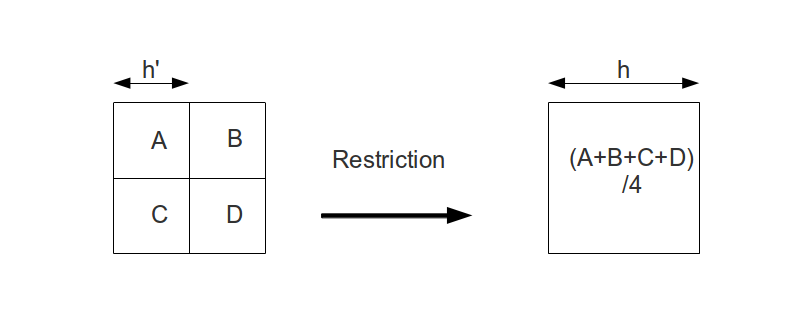
\includegraphics[width=.45\linewidth]{img/02/Restriction.png}}
\subfloat[Prolongation]{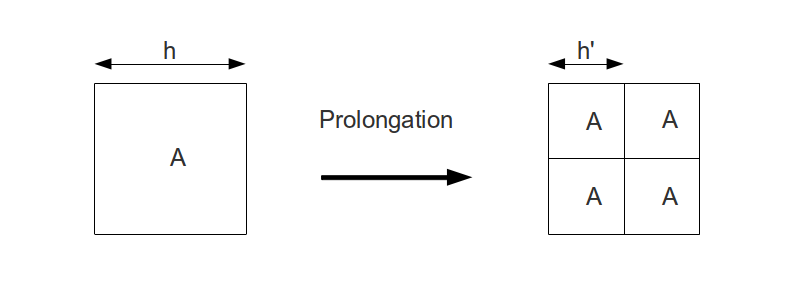
\includegraphics[width=.45\linewidth]{img/02/Prolongation.png}}\\
\subfloat[Niveau L  ]{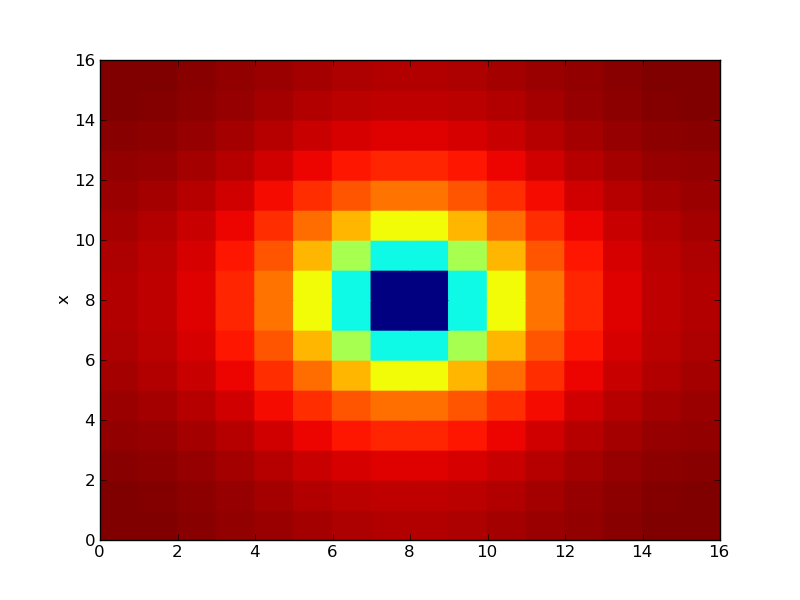
\includegraphics[width=.45\linewidth]{img/02/0090.png} \label{Opérateurs de changement de grille d}}
\subfloat[Niveau L+1]{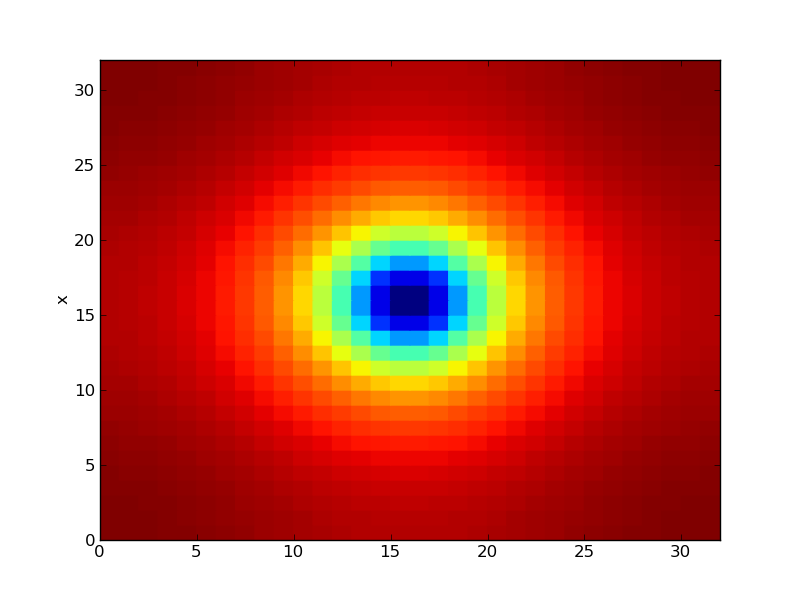
\includegraphics[width=.45\linewidth]{img/02/0088.png} \label{Opérateurs de changement de grille c}}
\caption[Opérateurs de changement de grille]{Opérateurs de changement de grille. 
Ils permettent de changer la résolution de la grille. 
Un exemple de restriction consiste à moyenner une valeur de plusieurs cellules, la prolongation associée consiste en une injection directe d'une valeur dans plusieurs cellules.
\label{Opérateurs de changement de grille}}
\end{center}
\end{figure}

%La prolongation et la restriction sont des opérateurs aisément parallélisables. Chaque cellule (ou paquet de huit cellules) est indépendante des autres et il est possible de ne changer la résolution que d'une partie de la grille sans en affecter le reste.

%Il existe principalement deux conditions sur les opérateurs de changement de grille. 
%La première impose une certaine réciprocité entre eux, les opérateurs doivent être adjoints: il est nécessaire qu'après une prolongation, suivie d'une restriction la grille d'arrivée soit la même que la grille de départ. 
%L'inverse n'est pas nécessairement vrai: après une restriction, de l'information est perdue et aucune prolongation ne pourra la recomposer.
%La seconde condition concerne la precision des opérateurs, il est nécessaire que la somme des ordres des opérations soit supérieure à l'ordre de l'équation à résoudre. 
%Ici, la restriction est d'ordre trois, la prolongation d'ordre un et le Laplacien d'ordre deux, cette condition est vérifiée.


\subsection{Recherche de voisins}
\label{sec:voisins}

Les processus physiques que l'on cherche à résoudre sont régis par des systèmes d'équations différentielles. (voir section \ref{sec:solvers})
En analyse numérique, une dérivée de $u$ suivant $x$ est localement approximée (dans le cas d'une différence finie centrée) par une équation de la forme :
\begin{equation}
\frac{d u}{dx} \approx \frac{u_{i+1}  - u_{i-1}}{2\Delta x}, 
\end{equation}
où $i$ est l'indice de la cellule appartenant à une grille régulière de pas $\Delta x$.
Dans ce type de systèmes, l'état d'une cellule dépend donc des états des cellules qui l'entourent.

La recherche de voisins est donc une étape importante dans la gestion de la grille qui a ici une organisation complexe (voir figure \ref{fig:octcell}).
Elle se fera en suivant les étapes présentées sur la figure \ref{fig:voisin}.
Dans le cas où la voisine se trouve dans le même OCT la recherche est immédiate.
Mais dans le cas ou la voisine n'est pas dans le même OCT, il faut trouver l'OCT voisin, vérifier que celui ci est géré par le même processus et vérifier si il est raffiné.
Cette recherche peut être complexe et numériquement coûteuse, on prendra donc garde à minimiser les appels de la fonction de recherche. 

\begin{figure}
        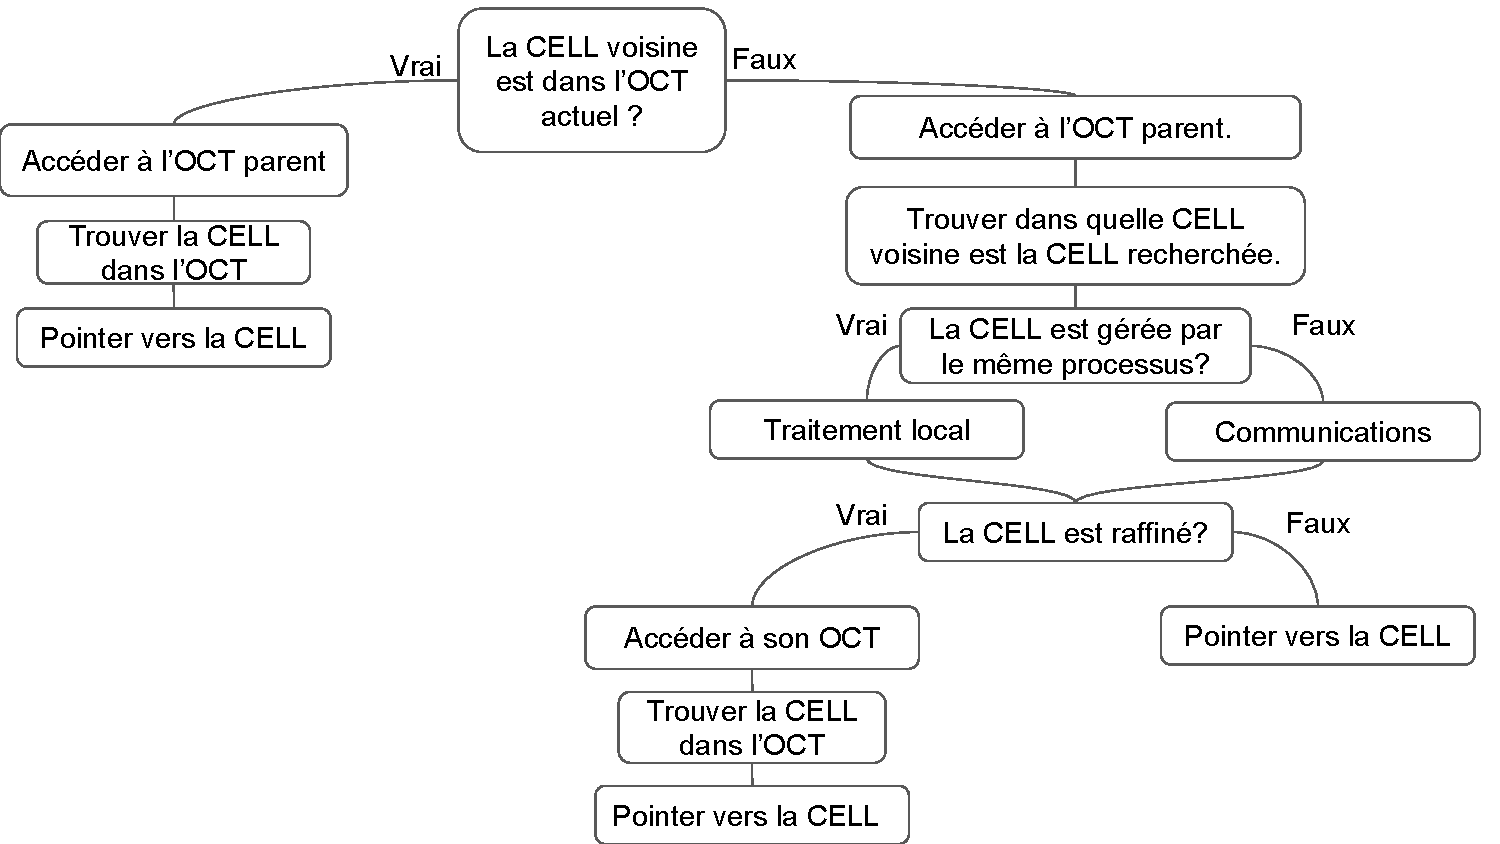
\includegraphics[width=\linewidth]{img/02/voisins.pdf} 
        \caption[Recherche de voisin dans l'octree.]{Arbre décisionnel pour la recherche de voisin dans l'octree.
        La recherche de voisins n'est pas triviale et peu avoir un coût non négligeable.
     	\label{fig:voisin} }
\end{figure}

%\begin{itemize}
%\item en fonction de l'ID de la cellule courante, déterminer si la voisine recherchée est dans le même OCT parent.
%
%\item
%\begin{itemize}
%\item Si c'est le cas: accéder à l'OCT parent, et à l'aide de l'indice du tableau de cellule, retrouver le voisin en question.
%\item Si ce n'est pas le cas, accéder à l'OCT parent, à l'aide des pointeurs sur les voisins, localiser l'OCT voisin et s'y rendre. Si l'OCT est raffiné déterminer 
%\end{itemize}
%
%\end{itemize}